% =====================================================================
%  Calcul mental - version diffusable
%
%  Meme contenu que rappels_calcul_mental_6e_5e.tex : les deux documents
%  chargent _contenu_calcul_mental.tex. Ce qui change ici, et seulement
%  ici : ni nom d'auteur, ni etablissement, ni classe, ni annee.
%  Le niveau n'apparait que sous forme d'etiquette de programme
%  (\prog{6}, \prog{5}) posee sur chaque titre de partie.
%
%  Toute correction de CONTENU se fait dans _contenu_calcul_mental.tex,
%  jamais ici : les deux versions restent ainsi synchronisees.
% =====================================================================
\documentclass[11pt]{exam}
\usepackage{../../mypackages}
\usepackage{../../macros}

\usepackage{../../stylecours}   % encadres, exercices, palette, schemas

\title{Calcul mental : méthodes et exercices}
\author{}
\date{}

% Les metadonnees du PDF sont vidées elles aussi : sans cela, hyperref y
% recopierait le titre et l'auteur du document.
\hypersetup{pdfauthor={}, pdftitle={Calcul mental : méthodes et exercices},
            pdfsubject={}, pdfcreator={}}

\begin{document}
{\let\newpage\relax\maketitle}

\begin{aretenir}[title={À quoi sert ce document ?}]
Le calcul mental n'est pas un don : c'est un ensemble d'\textbf{astuces} qui reposent
toutes sur quelques propriétés des opérations. Une fois ces propriétés comprises,
la plupart des calculs deviennent rapides.

Chaque partie porte une étiquette qui indique la classe où la notion est
\textbf{au programme} --- ou consolidée, pour ce qui vient de l'école élémentaire
(références : les repères annuels de progression d'éduscol, cycles 3 et 4). Chaque
partie suit toujours le même plan :

\begin{compactitem}
\item la \textbf{théorie} (la règle et pourquoi elle fonctionne) ;
\item plusieurs \textbf{exemples} résolus, détaillés étape par étape ;
\item une série de calculs à faire, sous le titre \textbf{À vous de jouer}.
\end{compactitem}

\textbf{Consigne générale pour tous les exercices :} calculer \textbf{mentalement},
sans poser l'opération et sans calculatrice.
\end{aretenir}

\tableofcontents
\newpage

% =====================================================================
%  Calcul mental - LE CONTENU
%  Ce fichier ne se compile pas seul : il est appele par \input depuis
%  les deux documents qui l'habillent.
%    - rappels_calcul_mental_6e_5e.tex  : la version de classe
%    - calcul_mental_partage.tex        : la version diffusable
%  Toute correction de contenu se fait ICI, une seule fois.
% =====================================================================
% =====================================================================
\section[Les tables de multiplication]{Les tables de multiplication \prog{6}}
% =====================================================================

Aucune astuce de calcul mental ne compense des tables mal sues : toutes les méthodes
qui suivent s'appuient dessus. C'est donc par là qu'il faut commencer.

% ---------------------------------------------------------------------
\subsection{La table, classée par difficulté}

\begin{aretenir}[title={Comment lire cette table}]
Les cases sont colorées selon la difficulté du résultat à retrouver :

\begin{compactitem}
\item \pastille{facile} \textbf{Facile} : résultat connu par
      cœur, ou immédiat à retrouver (tables de $1$, $2$, $5$ et $10$).
\item \pastille{moyen} \textbf{Moyen} : demande un petit effort de
      mémoire.
\item \pastille{difficile} \textbf{Difficile} : les résultats les
      plus souvent oubliés.
\end{compactitem}
\end{aretenir}

\begin{center}
\renewcommand{\arraystretch}{1.4}
\begin{tabular}{|c||c|c|c|c|c|c|c|c|c|c|}
\hline
\cellcolor{gray!30}$\times$ & \cellcolor{gray!30}\textbf{1} & \cellcolor{gray!30}\textbf{2} & \cellcolor{gray!30}\textbf{3} & \cellcolor{gray!30}\textbf{4} & \cellcolor{gray!30}\textbf{5} & \cellcolor{gray!30}\textbf{6} & \cellcolor{gray!30}\textbf{7} & \cellcolor{gray!30}\textbf{8} & \cellcolor{gray!30}\textbf{9} & \cellcolor{gray!30}\textbf{10} \\
\hline\hline
\cellcolor{gray!30}\textbf{1} & \mc{1}{1}{1} & \mc{1}{2}{2} & \mc{1}{3}{3} & \mc{1}{4}{4} & \mc{1}{5}{5} & \mc{1}{6}{6} & \mc{1}{7}{7} & \mc{1}{8}{8} & \mc{1}{9}{9} & \mc{1}{10}{10} \\ \hline
\cellcolor{gray!30}\textbf{2} & \mc{2}{1}{2} & \mc{2}{2}{4} & \mc{2}{3}{6} & \mc{2}{4}{8} & \mc{2}{5}{10} & \mc{2}{6}{12} & \mc{2}{7}{14} & \mc{2}{8}{16} & \mc{2}{9}{18} & \mc{2}{10}{20} \\ \hline
\cellcolor{gray!30}\textbf{3} & \mc{3}{1}{3} & \mc{3}{2}{6} & \mc{3}{3}{9} & \mc{3}{4}{12} & \mc{3}{5}{15} & \mc{3}{6}{18} & \mc{3}{7}{21} & \mc{3}{8}{24} & \mc{3}{9}{27} & \mc{3}{10}{30} \\ \hline
\cellcolor{gray!30}\textbf{4} & \mc{4}{1}{4} & \mc{4}{2}{8} & \mc{4}{3}{12} & \mc{4}{4}{16} & \mc{4}{5}{20} & \mc{4}{6}{24} & \mc{4}{7}{28} & \mc{4}{8}{32} & \mc{4}{9}{36} & \mc{4}{10}{40} \\ \hline
\cellcolor{gray!30}\textbf{5} & \mc{5}{1}{5} & \mc{5}{2}{10} & \mc{5}{3}{15} & \mc{5}{4}{20} & \mc{5}{5}{25} & \mc{5}{6}{30} & \mc{5}{7}{35} & \mc{5}{8}{40} & \mc{5}{9}{45} & \mc{5}{10}{50} \\ \hline
\cellcolor{gray!30}\textbf{6} & \mc{6}{1}{6} & \mc{6}{2}{12} & \mc{6}{3}{18} & \mc{6}{4}{24} & \mc{6}{5}{30} & \mc{6}{6}{36} & \mc{6}{7}{42} & \mc{6}{8}{48} & \mc{6}{9}{54} & \mc{6}{10}{60} \\ \hline
\cellcolor{gray!30}\textbf{7} & \mc{7}{1}{7} & \mc{7}{2}{14} & \mc{7}{3}{21} & \mc{7}{4}{28} & \mc{7}{5}{35} & \mc{7}{6}{42} & \mc{7}{7}{49} & \mc{7}{8}{56} & \mc{7}{9}{63} & \mc{7}{10}{70} \\ \hline
\cellcolor{gray!30}\textbf{8} & \mc{8}{1}{8} & \mc{8}{2}{16} & \mc{8}{3}{24} & \mc{8}{4}{32} & \mc{8}{5}{40} & \mc{8}{6}{48} & \mc{8}{7}{56} & \mc{8}{8}{64} & \mc{8}{9}{72} & \mc{8}{10}{80} \\ \hline
\cellcolor{gray!30}\textbf{9} & \mc{9}{1}{9} & \mc{9}{2}{18} & \mc{9}{3}{27} & \mc{9}{4}{36} & \mc{9}{5}{45} & \mc{9}{6}{54} & \mc{9}{7}{63} & \mc{9}{8}{72} & \mc{9}{9}{81} & \mc{9}{10}{90} \\ \hline
\cellcolor{gray!30}\textbf{10} & \mc{10}{1}{10} & \mc{10}{2}{20} & \mc{10}{3}{30} & \mc{10}{4}{40} & \mc{10}{5}{50} & \mc{10}{6}{60} & \mc{10}{7}{70} & \mc{10}{8}{80} & \mc{10}{9}{90} & \mc{10}{10}{100} \\ \hline
\end{tabular}
\end{center}

% ---------------------------------------------------------------------
\subsection{Les dix produits qui posent vraiment problème}

\begin{aretenir}
En enlevant les tables faciles, les carrés et les symétriques ($6 \times 7$ et
$7 \times 6$, c'est le même produit), il ne reste que \textbf{dix} résultats à
sécuriser. Dix, ce n'est pas beaucoup.

\begin{center}
\renewcommand{\arraystretch}{1.5}
\begin{tabular}{|c|c|c|c|c|}
\hline
\rowcolor{difficile}
$4 \times 6 = 24$ & $4 \times 7 = 28$ & $4 \times 8 = 32$ & $4 \times 9 = 36$ & $6 \times 7 = 42$ \\
\hline
\rowcolor{difficile}
$6 \times 8 = 48$ & $6 \times 9 = 54$ & $7 \times 8 = 56$ & $7 \times 9 = 63$ & $8 \times 9 = 72$ \\
\hline
\end{tabular}
\end{center}
\end{aretenir}

\begin{astuce}
Chacun de ces dix produits peut aussi se \textbf{recalculer} en quelques secondes, avec
les méthodes des parties suivantes. Si le résultat ne vient pas, on ne reste pas
bloqué :

\begin{compactitem}
\item \textbf{multiplier par 4} : doubler deux fois. $7 \times 4$ :
      $7 \times 2 = 14$, puis $14 \times 2 = 28$.
\item \textbf{multiplier par 8} : doubler trois fois. $7 \times 8$ :
      $14$, puis $28$, puis $56$.
\item \textbf{multiplier par 9} : $\times 10$, puis enlever le nombre.
      $7 \times 9 = 70 - 7 = 63$ ; $6 \times 9 = 60 - 6 = 54$ ; $8 \times 9 = 80 - 8 = 72$.
\item \textbf{multiplier par 6} : $\times 5$, puis ajouter le nombre.
      $6 \times 7 = 35 + 7 = 42$, car $5 \times 7 = 35$.
\end{compactitem}
\end{astuce}

\begin{exemple}{Exemple}{deux façons de retrouver $6 \times 8$}
\textbf{En doublant trois fois} (car $8 = 2 \times 2 \times 2$) :
$6 \rightarrow 12 \rightarrow 24 \rightarrow 48$.

\textbf{En passant par la table de 5} (car $6 = 5 + 1$) :
$5 \times 8 = 40$, puis $40 + 8 = 48$.
\end{exemple}

\begin{exostrois}
\ex{$6 \times 7$}  & \ex{$8 \times 9$}  & \ex{$4 \times 8$} \\
\ex{$7 \times 9$}  & \ex{$6 \times 8$}  & \ex{$4 \times 7$} \\
\ex{$7 \times 8$}  & \ex{$4 \times 9$}  & \ex{$6 \times 9$} \\
\ex{$4 \times 6$}  & \ex{$7 \times 7$}  & \ex{$8 \times 8$} \\
\ex{$9 \times 9$}  & \ex{$6 \times 6$}  & \ex{$12 \times 7$} \\
\end{exostrois}

% =====================================================================
\section[Les propriétés qui autorisent les astuces]{Les propriétés qui autorisent les astuces \prog{6}}
% =====================================================================

Toutes les astuces des parties suivantes reposent sur quatre propriétés. Les
connaître évite d'apprendre des recettes par cœur sans comprendre pourquoi
elles marchent.

% ---------------------------------------------------------------------
\subsection{La commutativité}

\begin{theorie}
La \textbf{commutativité} est la propriété qui permet de \textbf{changer l'ordre
des termes} sans changer le résultat.

Elle s'applique à l'addition et à la multiplication :
\[ a + b = b + a \qquad\text{et}\qquad a \times b = b \times a \]

\textbf{Autrement dit :} on peut faire passer le 3\up{e} terme en 1\up{er}, le dernier
en premier, etc.
\end{theorie}

\begin{exemple}{Exemple 1}{la propriété elle-même}
\[ 2 + 3 = 3 + 2 = 5 \qquad\qquad 2 \times 3 = 3 \times 2 = 6 \]
\end{exemple}

\begin{exemple}{Exemple 2}{à quoi ça sert}
Pour calculer $17 + 48 + 3$, on change l'ordre pour rapprocher $17$ et $3$ :
\begin{align*}
  17 + 48 + 3 &= 17 + 3 + 48 &&\text{par commutativité} \\
              &= 20 + 48     &&\text{car } 17 + 3 = 20 \\
              &= 68.
\end{align*}
\end{exemple}

\begin{exemple}{Exemple 3}{avec une multiplication}
Pour calculer $25 \times 7 \times 4$, on rapproche $25$ et $4$ :
\begin{align*}
  25 \times 7 \times 4 &= 25 \times 4 \times 7 &&\text{par commutativité} \\
                       &= 100 \times 7         &&\text{car } 25 \times 4 = 100 \\
                       &= 700.
\end{align*}
\end{exemple}

\begin{attention}
La \textbf{soustraction} et la \textbf{division} ne sont \textbf{pas} commutatives :
\[ 10 - 2 = 8 \qquad\text{mais}\qquad 2 - 10 = -8 \qquad\text{donc}\qquad 10 - 2 \neq 2 - 10 \]
\[ 10 \div 2 = 5 \qquad\text{mais}\qquad 2 \div 10 = 0{,}2 \qquad\text{donc}\qquad 10 \div 2 \neq 2 \div 10 \]
\end{attention}

\begin{exos}
\ex{$8 + 37 + 2$}   & \ex{$50 \times 9 \times 2$} \\
\ex{$19 + 25 + 1$}  & \ex{$4 \times 17 \times 25$} \\
\ex{$6 + 88 + 4$}   & \ex{$2 \times 43 \times 5$} \\
\end{exos}

% ---------------------------------------------------------------------
\subsection{L'associativité}

\begin{theorie}
L'\textbf{associativité} est la propriété qui permet de \textbf{regrouper les termes
avec des parenthèses}, dans l'ordre que l'on veut, sans changer le résultat.

Elle s'applique à l'addition et à la multiplication :
\[ (a + b) + c = a + (b + c) \qquad\text{et}\qquad (a \times b) \times c = a \times (b \times c) \]

\textbf{Autrement dit :} on peut commencer par l'opération que l'on veut.
\end{theorie}

\begin{exemple}{Exemple 1}{la propriété elle-même}
\[
\begin{array}{rcl}
  (10 + 20) + 30 &=& 10 + (20 + 30) \\
  30 + 30        &=& 10 + 50 \\
  60             &=& 60
\end{array}
\qquad\qquad
\begin{array}{rcl}
  (10 \times 20) \times 30 &=& 10 \times (20 \times 30) \\
  200 \times 30            &=& 10 \times 600 \\
  6\,000                   &=& 6\,000
\end{array}
\]
\end{exemple}

\begin{exemple}{Exemple 2}{choisir le regroupement le plus commode}
Pour calculer $48 + 27 + 3$, il vaut mieux commencer par la fin :
\begin{align*}
  48 + 27 + 3 &= 48 + (27 + 3) &&\text{par associativité} \\
              &= 48 + 30       &&\text{car } 27 + 3 = 30 \\
              &= 78.
\end{align*}
\end{exemple}

\begin{exemple}{Exemple 3}{avec une multiplication}
\begin{align*}
  2 \times 35 \times 5 &= 2 \times (35 \times 5) &&\text{par associativité} \\
                       &= 2 \times 175           &&\text{car } 35 \times 5 = 175 \\
                       &= 350.
\end{align*}
\end{exemple}

\begin{attention}
La \textbf{soustraction} et la \textbf{division} ne sont \textbf{pas} associatives :
\[
\begin{array}{rcl}
  (30 - 20) - 10 &\overset{?}{=}& 30 - (20 - 10) \\
  10 - 10        &\overset{?}{=}& 30 - 10 \\
  0              &\neq& 20
\end{array}
\qquad\qquad
\begin{array}{rcl}
  (100 \div 20) \div 5 &\overset{?}{=}& 100 \div (20 \div 5) \\
  5 \div 5             &\overset{?}{=}& 100 \div 4 \\
  1                    &\neq& 25
\end{array}
\]
\end{attention}

\begin{exos}
\ex{$56 + 18 + 2$}    & \ex{$4 \times 25 \times 13$} \\
\ex{$125 + 45 + 55$}  & \ex{$5 \times 20 \times 7$} \\
\ex{$70 + 12 + 8$}    & \ex{$8 \times 125 \times 3$} \\
\end{exos}

% ---------------------------------------------------------------------
\subsection{Les éléments neutres}

\begin{theorie}
Un \textbf{élément neutre} est un nombre qui, lorsqu'on fait une opération avec lui,
laisse l'autre nombre inchangé.

\begin{compactitem}
\item Pour l'\textbf{addition} et la \textbf{soustraction}, l'élément neutre est $\mathbf{0}$.
\item Pour la \textbf{multiplication} et la \textbf{division}, l'élément neutre est $\mathbf{1}$.
\end{compactitem}
\end{theorie}

\begin{exemple}{Exemple 1}{les quatre opérations}
\[
\begin{array}{ll}
  3 + 0 = 3 & -62 + 0 = -62 \\
  5 - 0 = 5 & -14 - 0 = -14 \\
  15 \times 1 = 15 & \dfrac{2}{3} \times 1 = \dfrac{2}{3} \\[0.8em]
  8 \div 1 = 8 & \dfrac{3}{4} \div 1 = \dfrac{3}{4}
\end{array}
\]
\end{exemple}

\begin{exemple}{Exemple 2}{pourquoi c'est utile (à garder en tête pour les fractions)}
Multiplier par $1$ ne change pas la valeur d'un nombre, \textbf{mais peut changer son
écriture}. Or $\dfrac{2}{2} = 1$, donc :
\[ \frac{1}{2} = \frac{1}{2} \times 1 = \frac{1}{2} \times \frac{2}{2} = \frac{2}{4} \]
C'est exactement le mécanisme qui permet de mettre deux fractions au même
dénominateur (voir la partie \ref{part:fractions}).
\end{exemple}

\begin{exemple}{Exemple 3}{repérer un élément neutre caché}
\begin{align*}
  37 \times 0{,}5 \times 2 &= 37 \times (0{,}5 \times 2) &&\text{par associativité} \\
                           &= 37 \times 1                &&\text{car } 0{,}5 \times 2 = 1 \\
                           &= 37.
\end{align*}
\end{exemple}

\begin{exos}
\ex{$46 \times 0{,}25 \times 4$}  & \ex{$92 \times 0{,}1 \times 10$} \\
\ex{$78 \times 0{,}2 \times 5$}   & \ex{$13 \times 0{,}5 \times 2$} \\
\end{exos}

% ---------------------------------------------------------------------
\subsection{La distributivité}

\begin{theorie}
La \textbf{distributivité} permet de transformer une multiplication par une somme
en une somme de multiplications.

Pour tous nombres $k$, $a$ et $b$ :
\[ \boxed{\,k \times (a + b) = k \times a + k \times b\,} \qquad
   \boxed{\,k \times (a - b) = k \times a - k \times b\,} \]

Ce que disent ces deux égalités : le facteur $k$ passe sur \textbf{chacun} des deux
termes de la parenthèse. L'oublier sur le second est l'erreur la plus fréquente.
\distrib{k}{a}{b}
\end{theorie}

\begin{exemple}{Exemple 1}{ce que ça veut dire concrètement}
J'ai $6$ sachets de bonbons. Dans chaque sachet, il y a $3$ schtroumpfs et $4$ cocas.
Combien de bonbons au total ?

\begin{center}
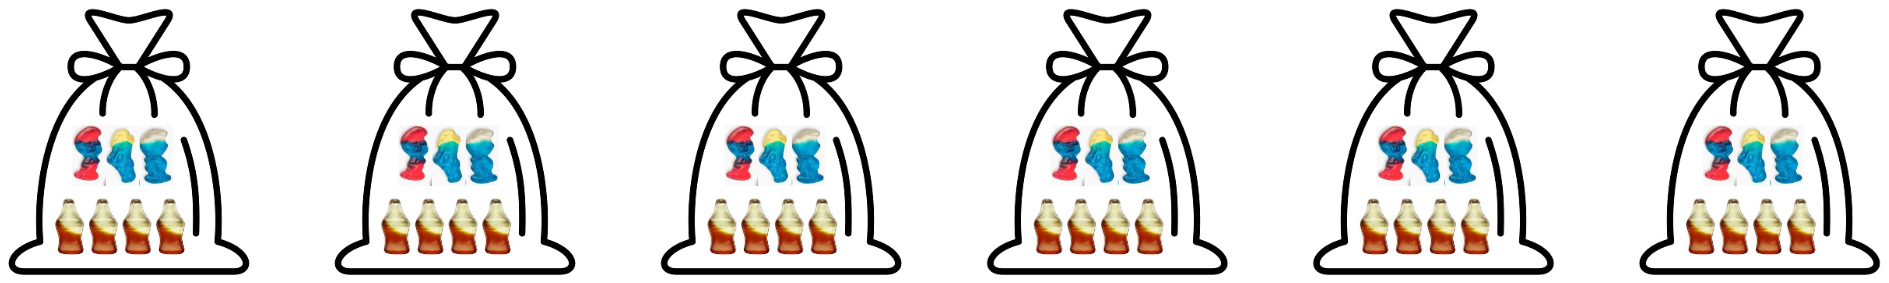
\includegraphics[width=0.94\linewidth]{figures/schema_sachets_distributivite.png}
\end{center}

\textbf{Option 1} : je compte les bonbons d'\underline{un} sachet, puis je multiplie par
le nombre de sachets.
\[ \text{Total} = 6 \times (3 + 4) = 6 \times 7 = 42 \]

\textbf{Option 2} : je compte tous les schtroumpfs, puis tous les cocas, et j'additionne.
\[ \text{Total} = 6 \times 3 + 6 \times 4 = 18 + 24 = 42 \]

Les deux façons donnent le même total, ce qui est exactement la distributivité :
\distrib{6}{3}{4}
\end{exemple}

\begin{exemple}{Exemple 2}{flèche par flèche, sur des nombres}
\distrib{12}{2}{3}
Il ne reste qu'à calculer les deux produits : $12 \times 2 = 24$ et
$12 \times 3 = 36$, donc $12 \times (2 + 3) = 60$.
\end{exemple}

\begin{exemple}{Exemple 3}{le cas qui servira tout le temps}
\begin{align*}
  8 \times 101 &= 8 \times (100 + 1)          &&\text{car } 101 = 100 + 1 \\
               &= 8 \times 100 + 8 \times 1   &&\text{par distributivité} \\
               &= 800 + 8 \\
               &= 808.
\end{align*}
\end{exemple}

\begin{exos}
\ex{$7 \times (10 + 3)$}   & \ex{$5 \times (20 - 1)$} \\
\ex{$4 \times (100 + 2)$}  & \ex{$9 \times (30 - 2)$} \\
\end{exos}

% =====================================================================
\section[Additionner et soustraire malin]{Additionner et soustraire malin \prog{6}}
% =====================================================================

% ---------------------------------------------------------------------
\subsection{La compensation : ajouter ou enlever 9, 99, 101\ldots}

\begin{astuce}
Les nombres proches d'une dizaine, d'une centaine ou d'un millier se traitent en
\textbf{deux temps} : on fait le calcul rond, puis on \textbf{compense}.

\begin{compactitem}
\item \textbf{Ajouter 299}, c'est ajouter $300$, puis enlever $1$.
\item \textbf{Enlever 19}, c'est enlever $20$, puis ajouter $1$.
\end{compactitem}
\end{astuce}

\begin{theorie}
Tout part d'une réécriture du nombre : $299 = 300 - 1$, $101 = 100 + 1$,
$999 = 1\,000 - 1$. Ce qui se passe ensuite dépend de l'opération.

\textbf{Quand on ajoute}, on enchaîne les deux étapes dans l'ordre, car l'addition
est associative :
\[ n + 299 = n + (300 - 1) = n + 300 - 1 \]

\textbf{Quand on soustrait}, le signe change devant la parenthèse : soustraire
$(100 - 1)$, c'est soustraire $100$ \emph{puis rajouter} $1$.
\[ n - 99 = n - (100 - 1) = n - 100 + 1 \]
\end{theorie}

\begin{exemple}{Exemple 1}{$2\,658 + 299$}
\compensation{2\,658 + 299}{2\,957}{2\,958}{+\,300}{-\,1}
\end{exemple}

\begin{exemple}{Exemple 2}{$374 - 99$}
\compensation{374 - 99}{275}{274}{-\,100}{+\,1}
\end{exemple}

\begin{exemple}{Exemple 3}{$63 + 101$}
\compensation{63 + 101}{164}{163}{+\,100}{+\,1}
\end{exemple}

\begin{aretenir}[title={Le tableau des compensations}]
\begin{center}
\renewcommand{\arraystretch}{1.4}
\begin{tabular}{|c|c|c||c|c|c|}
\hline
\rowcolor{entete}
\textbf{Opération} & \textbf{1\up{re} étape} & \textbf{2\up{e} étape} &
\textbf{Opération} & \textbf{1\up{re} étape} & \textbf{2\up{e} étape} \\
\hline
$+\,9$    & $+\,10$    & $-\,1$ & $-\,9$    & $-\,10$    & $+\,1$ \\ \hline
$+\,99$   & $+\,100$   & $-\,1$ & $-\,99$   & $-\,100$   & $+\,1$ \\ \hline
$+\,999$  & $+\,1\,000$& $-\,1$ & $-\,999$  & $-\,1\,000$& $+\,1$ \\ \hline
$+\,11$   & $+\,10$    & $+\,1$ & $-\,11$   & $-\,10$    & $-\,1$ \\ \hline
$+\,101$  & $+\,100$   & $+\,1$ & $-\,101$  & $-\,100$   & $-\,1$ \\ \hline
$+\,1\,001$& $+\,1\,000$& $+\,1$& $-\,1\,001$& $-\,1\,000$& $-\,1$ \\ \hline
\end{tabular}
\end{center}

Le même raisonnement marche avec $199$, $299$, $399\ldots$ (arrondir à $200$, $300$,
$400$ puis enlever $1$) et avec $201$, $301\ldots$ (arrondir puis ajouter $1$).
\end{aretenir}

\begin{exos}
\ex{$234 + 99$}        & \ex{$1\,289 - 101$} \\
\ex{$858 - 99$}        & \ex{$2\,658 + 299$} \\
\ex{$1\,263 + 101$}    & \ex{$3\,974 - 1\,001$} \\
\ex{$8\,127 + 799$}    & \ex{$1\,828 - 399$} \\
\ex{$3\,504 - 201$}    & \ex{$9\,368 + 599$} \\
\end{exos}

% ---------------------------------------------------------------------
\subsection{Le regroupement astucieux (addition)}

\begin{theorie}
Le regroupement astucieux consiste à utiliser la \textbf{commutativité} (je change
l'ordre des termes) et l'\textbf{associativité} (je commence par ce qui m'arrange)
pour arriver plus vite au résultat.

\textbf{On ne doit pas avoir à poser le calcul.}
\end{theorie}

\begin{astuce}
Deux réflexes :
\begin{compactenum}
\item Chercher les termes qui, ensemble, donnent un nombre \textbf{rond} : $10$, $100$,
      $1\,000$, ou un multiple de $10$.
\item Repérer tout de suite le terme \textbf{compliqué} et le garder pour la
      \textbf{dernière} opération.
\end{compactenum}
\end{astuce}

\begin{aretenir}[title={Les compléments à 10 : à connaître par cœur}]
\begin{center}
\renewcommand{\arraystretch}{1.3}
\begin{tabular}{|c|c|c|c|c|}
\hline
\rowcolor{entete}
$1 + 9$ & $2 + 8$ & $3 + 7$ & $4 + 6$ & $5 + 5$ \\
\hline
$10$ & $10$ & $10$ & $10$ & $10$ \\
\hline
\end{tabular}
\end{center}

Conséquence directe, valable quelle que soit la taille des nombres : un nombre qui
se termine par $\mathbf{1}$ se combine bien avec un nombre qui se termine par
$\mathbf{9}$, un qui finit par $\mathbf{2}$ avec un qui finit par $\mathbf{8}$, et ainsi
de suite.
\end{aretenir}

\begin{exemple}{Exemple 1}{avec des entiers}
\begin{align*}
  33 + 7 + 3 + 17 &= (33 + 17) + (7 + 3) &&\text{on rapproche les compléments} \\
                  &= 50 + 10 \\
                  &= 60.
\end{align*}
\end{exemple}

\begin{exemple}{Exemple 2}{avec des décimaux}
Avec des décimaux, on cherche les termes dont la somme donne un \textbf{entier}.
\begin{align*}
  21 + 3{,}1 + 79 + 0{,}9 &= 21 + 79 + 3{,}1 + 0{,}9 &&\text{par commutativité} \\
                          &= (21 + 79) + (3{,}1 + 0{,}9) &&\text{par associativité} \\
                          &= 100 + 4 \\
                          &= 104.
\end{align*}
\end{exemple}

\begin{exemple}{Exemple 3}{garder le terme compliqué pour la fin}
Dans $15 + 2{,}7 + 0{,}3 + 8$, le terme le moins commode est $2{,}7$ : on le laisse
se combiner avec $0{,}3$.
\begin{align*}
  15 + 2{,}7 + 0{,}3 + 8 &= (2{,}7 + 0{,}3) + 15 + 8 \\
                         &= 3 + 15 + 8 \\
                         &= 26.
\end{align*}
\end{exemple}

\begin{exos}
\ex{$7 + 3 + 12$}                & \ex{$37 + 3 + 40$} \\
\ex{$14 + 6 + 11 + 9$}           & \ex{$50 + 25 + 12 + 8$} \\
\ex{$5 + 15 + 25 + 8 + 2$}       & \ex{$90 + 4 + 6 + 10$} \\
\ex{$20 + 4{,}6 + 0{,}4 + 5$}    & \ex{$25 + 8{,}9 + 0{,}1 + 6$} \\
\ex{$7 + 12{,}5 + 0{,}5 + 3$}    & \ex{$6 + 23{,}75 + 0{,}25 + 12$} \\
\end{exos}

% =====================================================================
\section[Multiplier et diviser malin]{Multiplier et diviser malin \prog{6}}
% =====================================================================

% ---------------------------------------------------------------------
\subsection{Multiplier et diviser par 10, 100, 1\,000}

\begin{astuce}
Multiplier ou diviser par $10$, $100$, $1\,000$ revient à \textbf{décaler la virgule}
d'autant de rangs qu'il y a de zéros :
\begin{compactitem}
\item on décale vers la \textbf{droite} quand on \textbf{multiplie} (le nombre grandit) ;
\item on décale vers la \textbf{gauche} quand on \textbf{divise} (le nombre diminue).
\end{compactitem}
\end{astuce}

\begin{theorie}
Cette règle vient du fait que multiplier par $1\,000$, c'est multiplier trois fois
par $10$ :
\[ n \times 1\,000 = n \times 10 \times 10 \times 10 \]
et à chaque multiplication par $10$, la virgule avance d'un rang.
\end{theorie}

\begin{exemple}{Exemple 1}{$2{,}58 \times 1\,000$}
\begin{align*}
  2{,}58 \times 1\,000 &= 2{,}58 \times 10 \times 10 \times 10 &&\text{car } 1\,000 = 10 \times 10 \times 10 \\
                       &= 25{,}8 \times 10 \times 10           &&\text{la virgule avance d'un rang} \\
                       &= 258 \times 10                        &&\text{elle avance d'un deuxième rang} \\
                       &= 2\,580.                              &&\text{elle avance d'un troisième rang}
\end{align*}
\end{exemple}

\begin{exemple}{Exemple 2}{$897 \div 1\,000$}
Le nombre $897$ peut s'écrire $897{,}0$.
\begin{align*}
  897 \div 1\,000 &= 897{,}0 \div 10 \div 10 \div 10 \\
                  &= 89{,}7 \div 10 \div 10 &&\text{la virgule recule d'un rang} \\
                  &= 8{,}97 \div 10         &&\text{elle recule d'un deuxième rang} \\
                  &= 0{,}897.               &&\text{elle recule d'un troisième rang}
\end{align*}
\end{exemple}

\begin{exemple}{Exemple 3}{$0{,}0000237 \times 1\,000$}
Trois zéros, donc trois rangs vers la droite :
\[ 0{,}0000237 \times 1\,000 = 0{,}0237. \]
\end{exemple}

\begin{attention}
Quand on \textbf{divise}, le résultat est forcément \textbf{plus petit} que le nombre
de départ.

$187 \div 100$ revient à se demander : si je partage $187$\euro{} entre $100$ personnes,
combien reçoit chaque personne ? Forcément bien moins que $187$\euro{}. Le résultat
ne peut donc pas être $1\,870$ : il vaut $1{,}87$.

Prendre du recul sur l'ordre de grandeur du résultat évite cette erreur (voir la
partie \ref{part:controle}).
\end{attention}

\begin{exos}
\ex{$52 \div 10$}          & \ex{$52 \times 10$} \\
\ex{$452{,}3 \div 100$}    & \ex{$356 \times 1\,000$} \\
\ex{$22{,}2 \div 1\,000$}  & \ex{$7{,}652 \times 100$} \\
\ex{$84\,162 \div 100$}    & \ex{$2{,}45 \times 1\,000$} \\
\ex{$0{,}37 \div 100$}     & \ex{$0{,}0192017 \times 100$} \\
\end{exos}

% ---------------------------------------------------------------------
\subsection{Multiplier et diviser par 4}

\begin{astuce}
\begin{compactitem}
\item \textbf{Multiplier par 4}, c'est multiplier par $2$, puis encore par $2$
      (donc \textbf{doubler deux fois}).
\item \textbf{Diviser par 4}, c'est diviser par $2$, puis encore par $2$
      (donc prendre \textbf{deux fois la moitié}).
\end{compactitem}
\end{astuce}

\begin{theorie}
Cette astuce repose sur l'associativité et sur le fait que $4 = 2 \times 2$ :
\[ n \times 4 = n \times (2 \times 2) = (n \times 2) \times 2 \qquad\text{et}\qquad
   n \div 4 = n \div (2 \times 2) = (n \div 2) \div 2 \]
\end{theorie}

\fig{0.95}{figures/manuel_mult_div_4}{}

\begin{exemple}{Exemple 1}{$41 \times 4$}
\begin{align*}
  41 \times 4 &= 41 \times (2 \times 2) &&\text{on remplace } 4 \text{ par } 2 \times 2 \\
              &= (41 \times 2) \times 2 &&\text{par associativité} \\
              &= 82 \times 2            &&\text{car } 41 \times 2 = 82 \\
              &= 164.
\end{align*}
\end{exemple}

\begin{exemple}{Exemple 2}{$284 \div 4$}
\begin{align*}
  284 \div 4 &= (284 \div 2) \div 2 &&\text{on divise deux fois par } 2 \\
             &= 142 \div 2          &&\text{car } 284 \div 2 = 142 \\
             &= 71.
\end{align*}
\end{exemple}

\begin{exemple}{Exemple 3}{$117 \times 4$ (avec un nombre impair)}
\begin{align*}
  117 \times 4 &= (117 \times 2) \times 2 \\
               &= 234 \times 2 \\
               &= 468.
\end{align*}
\end{exemple}

\begin{exos}
\ex{$23 \times 4$}   & \ex{$92 \div 4$} \\
\ex{$27 \times 4$}   & \ex{$104 \div 4$} \\
\ex{$34 \times 4$}   & \ex{$132 \div 4$} \\
\ex{$19 \times 4$}   & \ex{$428 \div 4$} \\
\ex{$125 \times 4$}  & \ex{$12\,004 \div 4$} \\
\end{exos}

% ---------------------------------------------------------------------
\subsection{Multiplier et diviser par 5}

\begin{astuce}
\begin{compactitem}
\item \textbf{Multiplier par 5}, c'est multiplier par $10$, puis diviser par $2$.
\item \textbf{Diviser par 5}, c'est diviser par $10$, puis multiplier par $2$.
\end{compactitem}
\end{astuce}

\begin{theorie}
L'astuce vient de $5 = 10 \div 2$. Donc, pour n'importe quel nombre $x$ :
\[ x \times 5 = x \times 10 \div 2 \]

Pour la division, on peut le comprendre sans formule : \textbf{diviser par 5, c'est
faire des parts deux fois plus grandes que quand on divise par 10.} Pourquoi ? Parce
que $5$ est deux fois plus petit que $10$ : il y a deux fois moins de parts, donc
chaque part est deux fois plus grande. Et faire des parts deux fois plus grandes,
c'est multiplier par $2$ :
\[ x \div 5 = x \div (10 \div 2) = x \div 10 \times 2 \]
\end{theorie}

\fig{0.95}{figures/manuel_mult_div_5}{}

\begin{exemple}{Exemple 1}{$66 \times 5$}
\begin{align*}
  66 \times 5 &= 66 \times 10 \div 2 \\
              &= 660 \div 2 \\
              &= 330.
\end{align*}
\end{exemple}

\begin{exemple}{Exemple 2}{$160 \div 5$}
\begin{align*}
  160 \div 5 &= 160 \div 10 \times 2 \\
             &= 16 \times 2 \\
             &= 32.
\end{align*}
\end{exemple}

\begin{exemple}{Exemple 3}{$7{,}2 \times 5$ (avec un décimal)}
\begin{align*}
  7{,}2 \times 5 &= 7{,}2 \times 10 \div 2 \\
                 &= 72 \div 2 \\
                 &= 36.
\end{align*}
\end{exemple}

\begin{aretenir}[title={Les deux contrôles à faire systématiquement}]
\begin{compactenum}
\item Quand je \textbf{multiplie} par $5$, le résultat doit être \textbf{plus grand} que
      le nombre de départ (j'en ai $5$ fois plus).
\item Quand je \textbf{divise} par $5$, le résultat doit être \textbf{plus petit} que le
      nombre de départ (j'en ai $5$ fois moins).
\end{compactenum}

Et en cas de doute, on refait l'opération à l'envers. Par exemple, je trouve
$21 \times 5 = 105$. Je vérifie : $105 \div 5 = 105 \div 10 \times 2 = 10{,}5 \times 2 = 21$.
C'est bon.
\end{aretenir}

\begin{exos}
\ex{$32 \times 5$}      & \ex{$120 \div 5$} \\
\ex{$14 \times 5$}      & \ex{$40 \div 5$} \\
\ex{$0{,}6 \times 5$}   & \ex{$82 \div 5$} \\
\ex{$2{,}4 \times 5$}   & \ex{$1\,042 \div 5$} \\
\ex{$43{,}6 \times 5$}  & \ex{$53{,}7 \div 5$} \\
\ex{$27 \times 5$}      & \ex{$145 \div 5$} \\
\end{exos}

% ---------------------------------------------------------------------
\subsection{Le regroupement astucieux (multiplication)}

\begin{theorie}
Même principe que pour l'addition : on utilise la \textbf{commutativité} pour changer
l'ordre des facteurs et l'\textbf{associativité} pour commencer par ce qui arrange.

\textbf{On ne doit pas avoir à poser le calcul.} On repère le facteur compliqué et
on le garde pour la dernière opération.
\end{theorie}

\begin{aretenir}[title={Les produits à connaître par cœur}]
\begin{center}
\renewcommand{\arraystretch}{1.5}
\begin{tabular}{|c|c|c|}
\hline
\rowcolor{entete}
\multicolumn{3}{|c|}{\textbf{Les couples qui donnent un résultat rond}} \\
\hline
$0{,}5 \times 2 = 1$   & $0{,}25 \times 4 = 1$ & $0{,}2 \times 5 = 1$ \\ \hline
$0{,}1 \times 10 = 1$  & $0{,}5 \times 4 = 2$  & $2 \times 5 = 10$ \\ \hline
$2{,}5 \times 4 = 10$  & $2{,}5 \times 2 = 5$  & $0{,}125 \times 8 = 1$ \\ \hline
\end{tabular}
\end{center}
\end{aretenir}

\begin{exemple}{Exemple 1}{$2{,}5 \times 6{,}68 \times 4$}
Les facteurs à regrouper ($2{,}5$ et $4$) ne sont pas côte à côte : c'est justement
ce qu'il faut savoir repérer.
\begin{align*}
  2{,}5 \times 6{,}68 \times 4 &= (2{,}5 \times 4) \times 6{,}68 &&\text{par commutativité et associativité} \\
                               &= 10 \times 6{,}68               &&\text{car } 2{,}5 \times 4 = 10 \\
                               &= 66{,}8.
\end{align*}
\end{exemple}

\begin{exemple}{Exemple 2}{$0{,}5 \times 8{,}4 \times 4 \times 5$}
Ici, ce sont trois facteurs qui se regroupent : $0{,}5 \times 4 \times 5 = 10$.
\begin{align*}
  0{,}5 \times 8{,}4 \times 4 \times 5 &= (0{,}5 \times 4 \times 5) \times 8{,}4 \\
                                       &= (2 \times 5) \times 8{,}4 &&\text{car } 0{,}5 \times 4 = 2 \\
                                       &= 10 \times 8{,}4 \\
                                       &= 84.
\end{align*}
\end{exemple}

\begin{exemple}{Exemple 3}{$0{,}25 \times 78 \times 4$}
\begin{align*}
  0{,}25 \times 78 \times 4 &= (0{,}25 \times 4) \times 78 \\
                            &= 1 \times 78 &&\text{on retrouve l'élément neutre} \\
                            &= 78.
\end{align*}
\end{exemple}

\begin{exos}
\ex{$0{,}25 \times 67 \times 8$}      & \ex{$0{,}2 \times 45 \times 10$} \\
\ex{$0{,}5 \times 84 \times 2$}       & \ex{$0{,}2 \times 130 \times 100$} \\
\ex{$0{,}5 \times 246 \times 4$}      & \ex{$0{,}25 \times 17 \times 4$} \\
\ex{$0{,}1 \times 0{,}72 \times 1\,000$} & \ex{$0{,}2 \times 175 \times 5$} \\
\ex{$2{,}5 \times 6 \times 4 \times 2$}  & \ex{$0{,}5 \times 315 \times 2$} \\
\end{exos}

% ---------------------------------------------------------------------
\subsection{La distributivité en pratique : $\times\,8$, $\times\,9$, $\times\,11$, $\times\,98$, $\times\,101$}

\begin{theorie}
La distributivité dit que multiplier par une somme revient à multiplier par chaque
terme, puis à additionner :
\[ k \times (a + b) = k \times a + k \times b
   \qquad\qquad
   k \times (a - b) = k \times a - k \times b \]

En calcul mental, on s'en sert toujours de la même façon : on découpe le facteur
difficile en deux morceaux $a$ et $b$, choisis exprès pour que les deux
multiplications soient faciles.

\begin{compactitem}
\item $a$ est une \textbf{puissance de 10} ($10$, $100$, $1\,000$) : multiplier par $a$
      revient à décaler la virgule.
\item $b$ est un \textbf{tout petit nombre} ($1$ ou $2$) : multiplier par $b$ se fait
      de tête.
\end{compactitem}

Il ne reste plus qu'une addition ou une soustraction.
\end{theorie}

\begin{astuce}
Les découpages à repérer :

\begin{center}
\renewcommand{\arraystretch}{1.4}
\begin{tabular}{|c|c|c|c|c|}
\hline
\rowcolor{entete}
\multicolumn{5}{|c|}{$b = 1$} \\ \hline
$9 = 10 - 1$ & $11 = 10 + 1$ & $99 = 100 - 1$ & $101 = 100 + 1$ & $999 = 1\,000 - 1$ \\ \hline
\rowcolor{entete}
\multicolumn{5}{|c|}{$b = 2$} \\ \hline
$8 = 10 - 2$ & $12 = 10 + 2$ & $98 = 100 - 2$ & $102 = 100 + 2$ & $998 = 1\,000 - 2$ \\ \hline
\end{tabular}
\end{center}

Le facteur $k$, lui, ne doit pas être trop gros : il faut pouvoir faire l'addition
finale de tête. $43 \times 11$ est facile ($430 + 43$), $987 \times 11$ ne l'est pas.
\end{astuce}

\begin{exemple}{Exemple 1}{$43 \times 11$}
\begin{align*}
  43 \times 11 &= 43 \times (10 + 1)          &&\text{car } 11 = 10 + 1 \\
               &= 43 \times 10 + 43 \times 1  &&\text{par distributivité} \\
               &= 430 + 43 \\
               &= 473.
\end{align*}
\end{exemple}

\begin{exemple}{Exemple 2}{$63 \times 9$}
\begin{align*}
  63 \times 9 &= 63 \times (10 - 1)          &&\text{car } 9 = 10 - 1 \\
              &= 63 \times 10 - 63 \times 1  &&\text{par distributivité} \\
              &= 630 - 63 \\
              &= 567.
\end{align*}
\end{exemple}

\begin{exemple}{Exemple 3}{$4 \times 999$}
\begin{align*}
  4 \times 999 &= 4 \times (1\,000 - 1) \\
               &= 4\,000 - 4 \\
               &= 3\,996.
\end{align*}
\end{exemple}

\begin{exemple}{Exemple 4}{$25 \times 8$, un cas où $b = 2$}
Le facteur $8$ n'a l'air ni rond, ni proche de $10$. Et pourtant : $8 = 10 - 2$.
\begin{align*}
  25 \times 8 &= 25 \times (10 - 2)          &&\text{car } 8 = 10 - 2 \\
              &= 25 \times 10 - 25 \times 2  &&\text{par distributivité} \\
              &= 250 - 50 \\
              &= 200.
\end{align*}
\end{exemple}

\begin{exemple}{Exemple 5}{$45 \times 98$}
\begin{align*}
  45 \times 98 &= 45 \times (100 - 2)          &&\text{car } 98 = 100 - 2 \\
               &= 45 \times 100 - 45 \times 2  &&\text{par distributivité} \\
               &= 4\,500 - 90 \\
               &= 4\,410.
\end{align*}
\end{exemple}

\begin{aretenir}
La table de multiplication par $9$ fonctionne exactement sur ce principe :
\[ a \times 9 = a \times (10 - 1) = a \times 10 - a \]
Par exemple $7 \times 9 = 70 - 7 = 63$, et $8 \times 9 = 80 - 8 = 72$.
\end{aretenir}

\begin{exos}
\ex{$32 \times 101$}   & \ex{$60 \times 99$} \\
\ex{$30 \times 9$}     & \ex{$46 \times 11$} \\
\ex{$42 \times 102$}   & \ex{$5 \times 98$} \\
\ex{$31 \times 12$}    & \ex{$78 \times 8$} \\
\ex{$8 \times 1\,001$} & \ex{$17 \times 999$} \\
\ex{$45 \times 9$}     & \ex{$24 \times 11$} \\
\ex{$35 \times 8$}     & \ex{$15 \times 98$} \\
\ex{$12 \times 102$}   & \ex{$50 \times 12$} \\
\end{exos}

% =====================================================================
\section[L'ordre des opérations]{L'ordre des opérations \prog{6}}
% =====================================================================

\subsection{Les priorités de calcul}

\begin{theorie}
Dans un calcul qui mélange plusieurs opérations, on respecte toujours cet ordre :

\begin{compactenum}
\item les \textbf{parenthèses}, en commençant par les plus intérieures ;
\item les \textbf{multiplications} et les \textbf{divisions} ;
\item les \textbf{additions} et les \textbf{soustractions}.
\end{compactenum}

\textbf{Règle complémentaire, souvent oubliée :} une fois les multiplications et
divisions effectuées, les additions et soustractions restantes se calculent
\textbf{de gauche à droite}, dans l'ordre où elles sont écrites.
\end{theorie}

\begin{exemple}{Exemple 1}{repérer les multiplications}
\begin{align*}
  5 \times 4 - 3 \times 6 + 2 &= 20 - 18 + 2 &&\text{on fait d'abord les deux multiplications} \\
                              &= 2 + 2       &&\text{puis de gauche à droite : } 20 - 18 = 2 \\
                              &= 4.
\end{align*}
\end{exemple}

\begin{exemple}{Exemple 2}{des parenthèses imbriquées}
\begin{align*}
  25 + \bigl(7 - (3 + 2)\bigr) &= 25 + (7 - 5) &&\text{on calcule d'abord } (3+2) \\
                               &= 25 + 2 \\
                               &= 27.
\end{align*}
\end{exemple}

\begin{exemple}{Exemple 3}{une multiplication cachée dans une parenthèse}
\begin{align*}
  2 \times (3 + 8 \times 6) &= 2 \times (3 + 48) &&\text{dans la parenthèse, } \times \text{ d'abord} \\
                            &= 2 \times 51 \\
                            &= 102.
\end{align*}
\end{exemple}

\begin{attention}
Le piège classique est l'enchaînement \textbf{soustraction puis addition}. Dans
$18 - 3 \times 4 + 2$ :

\textcolor{atfr}{\textbf{Erreur fréquente}} : calculer $12 + 2 = 14$ puis $18 - 14 = 4$.

\textbf{Calcul correct} : on fait la multiplication, puis on avance de gauche à droite.
\[ 18 - 3 \times 4 + 2 = 18 - 12 + 2 = 6 + 2 = 8 \]

Il n'y a pas de parenthèse autour de $12 + 2$ : rien n'autorise à les regrouper.
\end{attention}

\begin{exos}
\ex{$2 + 3 \times 4$}                & \ex{$(9 - 3) \times (4 + 2)$} \\
\ex{$16 + 4 \times 2 + 5$}           & \ex{$77 - 2 \times 6 + 5$} \\
\ex{$18 + 4 - 3 \times 3$}           & \ex{$(12 - 3) \times 2 + 4$} \\
\ex{$3 \times (10 - 2) + (7 - 4)$}   & \ex{$(18 - 6) \times 2 + 3 \times 2$} \\
\ex{$3 \times \bigl((4 + 7) - 4 \times 2\bigr)$} & \ex{$53 - 6 \times (8 - 3)$} \\
\end{exos}

% =====================================================================
\section[Les pourcentages]{Les pourcentages \prog{6}}
% =====================================================================

\subsection{Calculer un pourcentage de tête}

\begin{theorie}
\textquotedbl{}$p\,\%$ de $X$\textquotedbl{} signifie
\[ \frac{p}{100} \times X. \]

Pour calculer de tête, on \textbf{simplifie la fraction} $\dfrac{p}{100}$ : elle se
ramène presque toujours à une division simple.
\end{theorie}

\begin{aretenir}[title={Le tableau des pourcentages de base}]
\begin{center}
\renewcommand{\arraystretch}{1.5}
% Colonnes m{} : centrage vertical sur toute la hauteur de la cellule. Avec des
% colonnes c, une fraction se cale sur l'axe mathématique et le texte voisin sur
% la ligne de base : les deux paraissent décalés l'un par rapport à l'autre.
% \rh : hauteur minimale de ligne. Sans elle, les lignes dont la 3e colonne tient
% en une seule ligne de texte sont trop basses et le \dfrac touche les filets.
\newcommand{\rh}{\rule[-1.5em]{0pt}{4em}}
\begin{tabular}{|>{\centering\arraybackslash}m{2.5cm}
                |>{\centering\arraybackslash}m{4.3cm}
                |>{\raggedright\arraybackslash}m{6.2cm}|}
\hline
\rowcolor{entete}
\centering\textbf{Pourcentage} & \centering\textbf{Le calcul} & \textbf{Ce que je fais} \\
\hline
\rh $50\,\%$ de $X$  & $\dfrac{1}{2} \times X = \dfrac{X}{2}$
                 & je divise $X$ par $2$ \\ \hline
\rh $25\,\%$ de $X$  & $\dfrac{1}{4} \times X = \dfrac{X}{4}$
                 & je divise $X$ par $4$, c'est-à-dire deux fois par $2$ \\ \hline
\rh $75\,\%$ de $X$  & $\dfrac{3}{4} \times X = \dfrac{3 \times X}{4}$
                 & je divise $X$ par $4$, puis je multiplie par $3$ \\ \hline
\rh $20\,\%$ de $X$  & $\dfrac{1}{5} \times X = \dfrac{X}{5}$
                 & je divise $X$ par $5$ \\ \hline
\rh $10\,\%$ de $X$  & $\dfrac{1}{10} \times X = \dfrac{X}{10}$
                 & je divise $X$ par $10$ \\ \hline
\rh $5\,\%$ de $X$   & $\dfrac{1}{20} \times X = \dfrac{X}{20}$
                 & je divise $X$ par $10$, puis je prends la moitié \\ \hline
\rh $1\,\%$ de $X$   & $\dfrac{1}{100} \times X = \dfrac{X}{100}$
                 & je divise $X$ par $100$ \\ \hline
\rh $40\,\%$ de $X$  & $\dfrac{2}{5} \times X = \dfrac{2 \times X}{5}$
                 & je divise $X$ par $5$, puis je multiplie par $2$ \\ \hline
\rh $80\,\%$ de $X$  & $\dfrac{4}{5} \times X = \dfrac{4 \times X}{5}$
                 & je divise $X$ par $5$, puis je multiplie par $4$ \\ \hline
\end{tabular}
\end{center}
\end{aretenir}

\begin{astuce}
Un pourcentage qui n'est pas dans le tableau se \textbf{décompose} :
\begin{compactitem}
\item par \textbf{addition} : $52\,\% = 50\,\% + 2\,\%$ ; $15\,\% = 10\,\% + 5\,\%$ ;
      $11\,\% = 10\,\% + 1\,\%$ ;
\item par \textbf{complément à 100} : $99\,\% = 100\,\% - 1\,\%$ ;
      $98\,\% = 100\,\% - 2\,\%$.
\end{compactitem}
\end{astuce}

\begin{theorie}
Ce qui autorise à couper le calcul en deux, c'est la \textbf{distributivité} :
\begin{align*}
  52\,\% \text{ de } X &= \frac{52}{100} \times X \\
                       &= \frac{(50 + 2) \times X}{100}          &&\text{car } 52 = 50 + 2 \\
                       &= \frac{50 \times X}{100} + \frac{2 \times X}{100}
                                                                 &&\text{par distributivité} \\
                       &= \frac{50}{100} \times X + \frac{2}{100} \times X \\
                       &= 50\,\% \text{ de } X \;+\; 2\,\% \text{ de } X.
\end{align*}

Le même raisonnement vaut pour le complément à $100$, avec une soustraction :
$98\,\%$ de $X = \dfrac{(100 - 2) \times X}{100} = X - 2\,\%$ de $X$.
\end{theorie}

\begin{exemple}{Exemple 1}{$25\,\%$ de $120$}
$25\,\% = \dfrac{1}{4}$, donc on divise par $4$, c'est-à-dire deux fois par $2$ :
\[ 120 \div 2 = 60, \qquad 60 \div 2 = 30. \qquad\text{Donc } 25\,\% \text{ de } 120 = 30. \]
\end{exemple}

\begin{exemple}{Exemple 2}{$52\,\%$ de $200$ (décomposition par addition)}
\begin{align*}
  52\,\% \text{ de } 200 &= 50\,\% \text{ de } 200 \;+\; 2\,\% \text{ de } 200 \\
                         &= 100 + 4 &&\text{car } 50\,\% \text{ c'est la moitié, et } 2\,\% = 2 \times 1\,\% \\
                         &= 104.
\end{align*}
\textbf{Contrôle} : $52\,\%$ est un peu plus que la moitié, donc le résultat doit être
un peu au-dessus de $100$. C'est cohérent.
\end{exemple}

\begin{exemple}{Exemple 3}{$98\,\%$ de $150$ (complément à 100)}
\begin{align*}
  98\,\% \text{ de } 150 &= 100\,\% \text{ de } 150 \;-\; 2\,\% \text{ de } 150 \\
                         &= 150 - 3 &&\text{car } 1\,\% \text{ de } 150 = 1{,}5 \text{ et } 2 \times 1{,}5 = 3 \\
                         &= 147.
\end{align*}
\end{exemple}

\begin{exos}
\ex{$50\,\%$ de $360$}   & \ex{$25\,\%$ de $160$} \\
\ex{$10\,\%$ de $542$}   & \ex{$20\,\%$ de $450$} \\
\ex{$75\,\%$ de $80$}    & \ex{$5\,\%$ de $60$} \\
\ex{$60\,\%$ de $200$}   & \ex{$15\,\%$ de $80$} \\
\ex{$99\,\%$ de $200$}   & \ex{$11\,\%$ de $300$} \\
\ex{$2\,\%$ de $400$}    & \ex{$80\,\%$ de $250$} \\
\end{exos}

% =====================================================================
\section[Les nombres relatifs]{Les nombres relatifs \prog{5}}
% =====================================================================

\subsection{Additionner et soustraire des nombres relatifs}

\begin{theorie}
Un \textbf{nombre relatif} se lit en deux morceaux : son \textbf{signe} ($+$ ou $-$) et sa
\textbf{distance à zéro}. Par exemple, $-7$ a pour signe $-$ et pour distance à zéro $7$.

\textbf{Pour additionner deux nombres relatifs :}
\begin{compactitem}
\item \textbf{mêmes signes} : on \textbf{additionne} les distances à zéro et on garde
      le signe commun ;
\item \textbf{signes contraires} : on \textbf{soustrait} la plus petite distance de la
      plus grande, et on garde le signe de celui qui est le plus loin de zéro.
\end{compactitem}

\textbf{Pour soustraire :} soustraire un nombre, c'est \textbf{ajouter son opposé}.
\[ \boxed{\,a - b = a + (-b)\,} \]
\end{theorie}

\begin{exemple}{Exemple 1}{mêmes signes, $(-7) + (-5)$}
Les deux nombres sont négatifs : j'additionne les distances ($7 + 5 = 12$) et je garde
le signe $-$.
\[ (-7) + (-5) = -12 \]
Sur une droite graduée, je recule de $7$, puis je recule encore de $5$ :
\begin{center}
\begin{tikzpicture}[>={Stealth[length=2.5mm]}, scale=0.70]
  \draw[->, thick] (-14.6,0) -- (2.6,0);
  \foreach \x in {-14,-12,-10,-8,-6,-4,-2,0,2}
    \draw (\x,0.14) -- (\x,-0.14) node[below=1pt, font=\scriptsize] {$\x$};
  \draw[->, very thick, exbleu] (0,0.2) to[bend right=40]
       node[midway, above=1pt, font=\small, fill=white, inner sep=1.5pt] {$-\,7$} (-7,0.2);
  \draw[->, very thick, atfr] (-7,0.2) to[bend right=40]
       node[midway, above=1pt, font=\small, fill=white, inner sep=1.5pt] {$-\,5$} (-12,0.2);
  \fill[exbleu] (-7,0) circle (2.6pt);
  \fill[atfr]   (-12,0) circle (2.6pt);
\end{tikzpicture}
\end{center}
\end{exemple}

\begin{exemple}{Exemple 2}{signes contraires, $(-7) + 4$}
Les signes sont contraires : je soustrais les distances ($7 - 4 = 3$) et je garde le
signe de $-7$, qui est le plus loin de zéro.
\[ (-7) + 4 = -3 \]
\end{exemple}

\begin{exemple}{Exemple 3}{une soustraction, $3 - 8$}
\begin{align*}
  3 - 8 &= 3 + (-8) &&\text{soustraire } 8 \text{, c'est ajouter } -8 \\
        &= -5       &&\text{signes contraires : } 8 - 3 = 5 \text{, et } -8 \text{ est le plus loin de } 0.
\end{align*}
\end{exemple}

\begin{exemple}{Exemple 4}{soustraire un négatif, $5 - (-3)$}
\begin{align*}
  5 - (-3) &= 5 + (+3) &&\text{l'opposé de } -3 \text{ est } +3 \\
           &= 8.
\end{align*}
Deux signes $-$ qui se suivent se transforment en $+$.
\end{exemple}

\begin{exemple}{Exemple 5}{les deux à la fois, $-4 - (-9)$}
\begin{align*}
  -4 - (-9) &= -4 + 9 \\
            &= 5      &&\text{signes contraires : } 9 - 4 = 5 \text{, et } +9 \text{ est le plus loin de } 0.
\end{align*}
\end{exemple}

\begin{attention}
Ne pas confondre le signe d'un nombre et le signe d'une opération.

Dans $-5 - 3$, il y a un nombre $-5$ \textbf{et} une soustraction. On recule donc encore :
\[ -5 - 3 = -5 + (-3) = -8 \qquad\text{(et non } -2\text{)}. \]

Le réflexe qui protège : se demander \textbf{de quel côté on va sur la droite graduée}.
Ajouter un positif fait avancer, ajouter un négatif fait reculer.
\end{attention}

\begin{exostrois}
\ex{$(-6) + (-9)$}  & \ex{$(-12) + 5$}   & \ex{$7 + (-15)$} \\
\ex{$4 - 11$}       & \ex{$-3 - 8$}      & \ex{$-20 + 20$} \\
\ex{$6 - (-4)$}     & \ex{$-7 - (-7)$}   & \ex{$-13 - (-5)$} \\
\ex{$-2{,}5 + 1{,}5$} & \ex{$-100 + 45$} & \ex{$18 - (-2)$} \\
\end{exostrois}

% =====================================================================
\section[Les fractions]{Les fractions \prog{5}}
\label{part:fractions}
% =====================================================================

% ---------------------------------------------------------------------
\subsection{Fractions égales et simplification}

\begin{theorie}
Multiplier (ou diviser) le numérateur \textbf{et} le dénominateur par un même nombre
non nul ne change pas la valeur de la fraction :
\[ \boxed{\;\frac{a}{b} = \frac{a \times k}{b \times k} = \frac{a \div k}{b \div k}\;} \]

C'est exactement l'élément neutre de la multiplication : $\dfrac{k}{k} = 1$, et
multiplier par $1$ ne change rien.
\end{theorie}

\begin{exemple}{Exemple 1}{simplifier $\dfrac{6}{8}$}
$6$ et $8$ sont tous les deux divisibles par $2$. On décompose, puis on barre le
facteur commun en haut et en bas :
\[ \frac{6}{8} = \frac{2 \times 3}{2 \times 4}
               = \frac{\cancel{2} \times 3}{\cancel{2} \times 4}
               = \frac{3}{4}. \]
\end{exemple}

\begin{exemple}{Exemple 2}{simplifier $\dfrac{24}{36}$ en plusieurs étapes}
Inutile de chercher le bon diviseur du premier coup : on enchaîne les petites
simplifications jusqu'à ne plus pouvoir. À chaque étape, on décompose et on barre.
\begin{align*}
  \frac{24}{36} &= \frac{\cancel{2} \times 12}{\cancel{2} \times 18} = \frac{12}{18} \\[0.3em]
                &= \frac{\cancel{2} \times 6}{\cancel{2} \times 9}   = \frac{6}{9}   \\[0.3em]
                &= \frac{\cancel{3} \times 2}{\cancel{3} \times 3}   = \frac{2}{3}.
\end{align*}
À chaque étape, on se demande simplement si les deux nombres sont pairs, puis s'ils
sont dans la table de $3$.
\end{exemple}

\begin{exemple}{Exemple 3}{reconnaître deux fractions égales}
$\dfrac{3}{5}$ et $\dfrac{15}{25}$ sont-elles égales ? Oui :
\[ \frac{15}{25} = \frac{5 \times 3}{5 \times 5}
                 = \frac{\cancel{5} \times 3}{\cancel{5} \times 5}
                 = \frac{3}{5}. \]
\end{exemple}

\begin{aretenir}[title={Les équivalences à connaître par cœur}]
\begin{center}
\renewcommand{\arraystretch}{1.4}
% Colonnes m{} et hauteur minimale garantie : voir le tableau des pourcentages.
\newcommand{\rhb}{\rule[-1.5em]{0pt}{4em}}
\begin{tabular}{|>{\centering\arraybackslash}m{1.6cm}|>{\centering\arraybackslash}m{1.6cm}|>{\centering\arraybackslash}m{2.5cm}
                ||>{\centering\arraybackslash}m{1.6cm}|>{\centering\arraybackslash}m{1.6cm}|>{\centering\arraybackslash}m{2.5cm}|}
\hline
\rowcolor{entete}
\centering\textbf{Fraction} & \centering\textbf{Décimal} & \centering\textbf{Pourcentage} &
\centering\textbf{Fraction} & \centering\textbf{Décimal} & \textbf{Pourcentage} \\
\hline
\rhb $\dfrac{1}{2}$ & $0{,}5$   & $50\,\%$     & $\dfrac{1}{5}$   & $0{,}2$  & $20\,\%$ \\ \hline
\rhb $\dfrac{1}{4}$ & $0{,}25$  & $25\,\%$     & $\dfrac{2}{5}$   & $0{,}4$  & $40\,\%$ \\ \hline
\rhb $\dfrac{3}{4}$ & $0{,}75$  & $75\,\%$     & $\dfrac{1}{10}$  & $0{,}1$  & $10\,\%$ \\ \hline
\rhb $\dfrac{1}{8}$ & $0{,}125$ & $12{,}5\,\%$ & $\dfrac{1}{100}$ & $0{,}01$ & $1\,\%$ \\ \hline
\end{tabular}
\end{center}

Le cas de $\dfrac{1}{3}$ est à part : son écriture décimale ne s'arrête jamais
($0{,}333\ldots$). On le laisse en fraction.
\end{aretenir}

\begin{exostrois}[3.2]
\ex{$\dfrac{10}{15}$}  & \ex{$\dfrac{9}{12}$}   & \ex{$\dfrac{14}{21}$} \\
\ex{$\dfrac{45}{60}$}  & \ex{$\dfrac{16}{40}$}  & \ex{$\dfrac{35}{100}$} \\
\end{exostrois}

% ---------------------------------------------------------------------
\subsection{Additionner et soustraire des fractions}

\begin{theorie}
\textbf{Si les dénominateurs sont les mêmes}, on additionne (ou soustrait) les
numérateurs et on garde le dénominateur :
\[ \frac{a}{d} + \frac{b}{d} = \frac{a + b}{d} \]

\textbf{S'ils sont différents}, on met d'abord les fractions au \textbf{même dénominateur},
en multipliant numérateur et dénominateur par le même nombre.
\end{theorie}

\begin{astuce}
Le cas le plus fréquent, et le plus rapide de tête : quand \textbf{un dénominateur est
un multiple de l'autre}. On ne transforme alors qu'\emph{une seule} des deux fractions.
\end{astuce}

\begin{exemple}{Exemple 1}{même dénominateur}
\[ \frac{3}{7} + \frac{2}{7} = \frac{3 + 2}{7} = \frac{5}{7}. \]
\end{exemple}

\begin{exemple}{Exemple 2}{un dénominateur multiple de l'autre}
Ici $4 = 2 \times 2$, donc on transforme seulement $\dfrac{1}{2}$ :
\begin{align*}
  \frac{1}{2} + \frac{1}{4} &= \frac{1 \times 2}{2 \times 2} + \frac{1}{4} \\
                            &= \frac{2}{4} + \frac{1}{4} \\
                            &= \frac{3}{4}.
\end{align*}
\end{exemple}

\begin{exemple}{Exemple 3}{une soustraction}
Ici $6 = 3 \times 2$, donc on transforme $\dfrac{1}{3}$ :
\begin{align*}
  \frac{5}{6} - \frac{1}{3} &= \frac{5}{6} - \frac{1 \times 2}{3 \times 2} \\
                            &= \frac{5}{6} - \frac{2}{6} \\
                            &= \frac{3}{6} = \frac{1}{2}. &&\text{on simplifie le résultat}
\end{align*}
\end{exemple}

\begin{exemple}{Exemple 4}{un entier plus une fraction}
Un entier s'écrit toujours comme une fraction de dénominateur $1$, donc :
\[ 2 + \frac{1}{3} = \frac{2 \times 3}{1 \times 3} + \frac{1}{3} = \frac{6}{3} + \frac{1}{3} = \frac{7}{3}. \]
\end{exemple}

\begin{attention}
On n'additionne \textbf{jamais} les dénominateurs entre eux :
\[ \frac{1}{2} + \frac{1}{4} \neq \frac{2}{6} \]

Le contrôle de bon sens : $\dfrac{1}{2}$ vaut déjà $0{,}5$, donc la somme doit être
\textbf{plus grande} que $0{,}5$. Or $\dfrac{2}{6}$ vaut environ $0{,}33$ : c'est
impossible. Le bon résultat est $\dfrac{3}{4}$, soit $0{,}75$.
\end{attention}

\begin{exos}[3.2]
\ex{$\dfrac{2}{9} + \dfrac{5}{9}$}    & \ex{$\dfrac{1}{3} + \dfrac{1}{6}$} \\
\ex{$\dfrac{7}{10} - \dfrac{3}{10}$}  & \ex{$\dfrac{3}{4} - \dfrac{1}{8}$} \\
\ex{$\dfrac{1}{2} + \dfrac{3}{10}$}   & \ex{$1 + \dfrac{2}{5}$} \\
\ex{$\dfrac{5}{6} + \dfrac{1}{2}$}    & \ex{$3 - \dfrac{1}{4}$} \\
\end{exos}

% ---------------------------------------------------------------------
\subsection{Multiplier des fractions}

\begin{theorie}
Pour multiplier deux fractions, on multiplie les numérateurs entre eux et les
dénominateurs entre eux :
\[ \boxed{\;\frac{a}{b} \times \frac{c}{d} = \frac{a \times c}{b \times d}\;} \]

Contrairement à l'addition, \textbf{aucun dénominateur commun n'est nécessaire}.
\end{theorie}

\begin{astuce}
\textbf{Simplifier avant de multiplier}, jamais après. Multiplier d'abord donne de
grands nombres qu'il faut ensuite simplifier péniblement.
\end{astuce}

\begin{exemple}{Exemple 1}{la règle}
\[ \frac{2}{3} \times \frac{4}{5} = \frac{2 \times 4}{3 \times 5} = \frac{8}{15}. \]
\end{exemple}

\begin{exemple}{Exemple 2}{simplifier avant de multiplier}
On décompose d'abord $9$ et $8$, pour faire apparaître en bas les facteurs qui sont
déjà en haut. On peut alors les barrer des deux côtés.
\begin{align*}
  \frac{4}{9} \times \frac{3}{8}
    &= \frac{4 \times 3}{9 \times 8} \\
    &= \frac{4 \times 3}{(3 \times 3) \times (4 \times 2)}
       &&\text{car } 9 = 3 \times 3 \text{ et } 8 = 4 \times 2 \\
    &= \frac{\cancel{4} \times \cancel{3}}{(\cancel{3} \times 3) \times (\cancel{4} \times 2)} \\
    &= \frac{1}{3 \times 2} \;=\; \frac{1}{6}.
\end{align*}
\end{exemple}

\begin{exemple}{Exemple 3}{un entier fois une fraction}
\[ 7 \times \frac{2}{7} = \frac{7}{1} \times \frac{2}{7}
   = \frac{7 \times 2}{7} = \frac{\cancel{7} \times 2}{\cancel{7}} = 2. \]
\end{exemple}

\begin{exemple}{Exemple 4}{le lien avec les pourcentages}
Prendre $\dfrac{3}{4}$ d'un nombre, c'est en prendre $75\,\%$ :
\[ \frac{3}{4} \times 80 = \frac{3 \times 80}{4} = \frac{240}{4} = 60, \]
ce qui est bien $75\,\%$ de $80$.
\end{exemple}

\begin{exos}[3.2]
\ex{$\dfrac{1}{2} \times \dfrac{3}{5}$}   & \ex{$\dfrac{5}{6} \times \dfrac{3}{10}$} \\
\ex{$\dfrac{2}{7} \times \dfrac{7}{3}$}   & \ex{$6 \times \dfrac{5}{12}$} \\
\ex{$\dfrac{3}{8} \times \dfrac{4}{9}$}   & \ex{$\dfrac{2}{5} \times 100$} \\
\end{exos}

% =====================================================================
\section[Vérifier son résultat]{Vérifier son résultat \prog{6}}
\label{part:controle}
% =====================================================================

Un calcul mental juste, c'est un calcul \textbf{contrôlé}. Les trois réflexes de cette
partie ne servent pas à trouver le résultat, mais à repérer qu'il est faux.

% ---------------------------------------------------------------------
\subsection{L'ordre de grandeur}

\begin{theorie}
Avant (ou après) le calcul, on \textbf{arrondit} les nombres pour estimer rapidement le
résultat attendu. Si le résultat trouvé est très loin de cette estimation, il y a
une erreur : virgule mal placée, zéro oublié, signe inversé.
\end{theorie}

\begin{exemple}{Exemple 1}{avec la distributivité}
\begin{center}
\renewcommand{\arraystretch}{1.5}
\begin{tabular}{|c|c|c|c|}
\hline
\rowcolor{entete}
\textbf{Opération} & \textbf{On arrondit} & \textbf{Estimation} & \textbf{Résultat exact} \\
\hline
$3 \times 999$    & $999 \approx 1\,000$   & $\approx 3\,000$ & $2\,997$ \\ \hline
$6 \times 101$    & $101 \approx 100$      & $\approx 600$    & $606$ \\ \hline
$4 \times 498$    & $498 \approx 500$      & $\approx 2\,000$ & $1\,992$ \\ \hline
$7 \times 52$     & $52 \approx 50$        & $\approx 350$    & $364$ \\ \hline
\end{tabular}
\end{center}
\end{exemple}

\begin{exemple}{Exemple 2}{avec les multiplications et divisions par 10, 100, 1\,000}
\begin{center}
\renewcommand{\arraystretch}{1.5}
\begin{tabular}{|c|c|c|c|}
\hline
\rowcolor{entete}
\textbf{Opération} & \textbf{On arrondit} & \textbf{Estimation} & \textbf{Résultat exact} \\
\hline
$42{,}47 \times 100$ & $42{,}47 \approx 40$ & $\approx 4\,000$ & $4\,247$ \\ \hline
$3{,}8 \times 1\,000$& $3{,}8 \approx 4$    & $\approx 4\,000$ & $3\,800$ \\ \hline
$874 \div 10$        & $874 \approx 900$    & $\approx 90$     & $87{,}4$ \\ \hline
$62 \div 1\,000$     & $62 \approx 60$      & $\approx 0{,}06$ & $0{,}062$ \\ \hline
\end{tabular}
\end{center}
\end{exemple}

\begin{exemple}{Exemple 3}{avec un pourcentage}
$52\,\%$ de $200$ : c'est un peu plus que la moitié de $200$, donc un peu plus de
$100$. On attend un résultat autour de $104$.
\end{exemple}

% ---------------------------------------------------------------------
\subsection{Le dernier chiffre et la parité}

\begin{attention}
Les règles de cette section ne valent que pour les \textbf{nombres entiers}. Avec des
décimaux, le \textquotedbl{}dernier chiffre\textquotedbl{} n'a pas le même sens : par exemple
$0{,}7 \times 10 = 7$, alors qu'on pourrait attendre un résultat finissant par $0$.
\end{attention}

\begin{theorie}
\textbf{Pour une multiplication comme pour une addition}, le dernier chiffre du
résultat ne dépend que des \textbf{chiffres des unités}. Il suffit donc de faire le
petit calcul sur ces deux chiffres.
\end{theorie}

\begin{exemple}{Exemple 1}{multiplications}
\begin{center}
\renewcommand{\arraystretch}{1.5}
\begin{tabular}{|l|l|l|}
\hline
\rowcolor{entete}
\textbf{Opération} & \textbf{Chiffres des unités} & \textbf{Dernier chiffre} \\
\hline
$3\textcolor{atfr}{7} \times 1\textcolor{atfr}{1} = 40\textcolor{atfr}{7}$ & $7 \times 1 = 7$   & finit par $\mathbf{7}$ \\ \hline
$1\textcolor{atfr}{3} \times 1\textcolor{atfr}{2} = 15\textcolor{atfr}{6}$ & $3 \times 2 = 6$   & finit par $\mathbf{6}$ \\ \hline
$\textcolor{atfr}{7} \times 1\textcolor{atfr}{6} = 11\textcolor{atfr}{2}$  & $7 \times 6 = 42$  & finit par $\mathbf{2}$ \\ \hline
\end{tabular}
\end{center}
\end{exemple}

\begin{exemple}{Exemple 2}{additions}
\begin{center}
\renewcommand{\arraystretch}{1.5}
\begin{tabular}{|l|l|l|}
\hline
\rowcolor{entete}
\textbf{Opération} & \textbf{Chiffres des unités} & \textbf{Dernier chiffre} \\
\hline
$22\textcolor{atfr}{4} + \textcolor{atfr}{8} = 23\textcolor{atfr}{2}$        & $4 + 8 = 12$ & finit par $\mathbf{2}$ \\ \hline
$15\textcolor{atfr}{7} + 3\textcolor{atfr}{6} = 19\textcolor{atfr}{3}$       & $7 + 6 = 13$ & finit par $\mathbf{3}$ \\ \hline
$48\textcolor{atfr}{9} + 4\textcolor{atfr}{7} = 53\textcolor{atfr}{6}$       & $9 + 7 = 16$ & finit par $\mathbf{6}$ \\ \hline
\end{tabular}
\end{center}
\end{exemple}

\begin{exemple}{Exemple 3}{anticiper le dernier chiffre d'une soustraction}
Le principe : chercher \textbf{quel chiffre, ajouté au chiffre qu'on soustrait, donne
le chiffre des unités du nombre de départ}.
\begin{compactitem}
\item $22\textcolor{atfr}{7} - \textcolor{atfr}{9}$ : quel chiffre ajouté à $9$ finit
      par $7$ ? On sait que $8 + 9 = 17$, donc le résultat finit par $\mathbf{8}$ :
      $227 - 9 = 218$.
\item $35\textcolor{atfr}{4} - 1\textcolor{atfr}{6}$ : quel chiffre ajouté à $6$ finit
      par $4$ ? On sait que $8 + 6 = 14$, donc le résultat finit par $\mathbf{8}$ :
      $354 - 16 = 338$.
\end{compactitem}
\end{exemple}

\begin{aretenir}[title={Pair ou impair ?}]
\begin{center}
\renewcommand{\arraystretch}{1.4}
\begin{tabular}{|c|l|l|}
\hline
\rowcolor{entete}
\textbf{Opération} & \textbf{Situation} & \textbf{Le résultat est\ldots} \\
\hline
\multirow{3}{*}{Addition} & Pair $+$ Pair       & toujours \textbf{pair} \quad (ex : $6 + 8 = 14$) \\ \cline{2-3}
 & Impair $+$ Impair & toujours \textbf{pair} \quad (ex : $7 + 9 = 16$) \\ \cline{2-3}
 & Pair $+$ Impair   & toujours \textbf{impair} \quad (ex : $6 + 7 = 13$) \\ \hline
\multirow{3}{*}{Soustraction} & Pair $-$ Pair   & toujours \textbf{pair} \quad (ex : $14 - 8 = 6$) \\ \cline{2-3}
 & Impair $-$ Impair & toujours \textbf{pair} \quad (ex : $17 - 9 = 8$) \\ \cline{2-3}
 & Pair $-$ Impair   & toujours \textbf{impair} \quad (ex : $14 - 7 = 7$) \\ \hline
\end{tabular}
\end{center}
\end{aretenir}

% ---------------------------------------------------------------------
\subsection{L'opération inverse}

\begin{theorie}
Une division se vérifie par une multiplication, et inversement :
\[ \text{si } a \div b = c \quad\text{alors}\quad c \times b = a. \]
\end{theorie}

\begin{exemple}{Exemple 1}{débusquer une erreur classique}
Je pense que $187 \div 100 = 1\,870$. Je vérifie :
\[ 1\,870 \times 100 = 187\,000 \neq 187. \]
C'est donc faux. Le bon résultat est $1{,}87$, et on a bien $1{,}87 \times 100 = 187$.
\end{exemple}

\begin{exemple}{Exemple 2}{vérifier une multiplication par 5}
Je calcule $21 \times 5 = 21 \times 10 \div 2 = 210 \div 2 = 105$.
Je vérifie à l'envers : $105 \div 5 = 105 \div 10 \times 2 = 10{,}5 \times 2 = 21$. C'est bon.
\end{exemple}

\begin{exemple}{Exemple 3}{contrôler une division sans la refaire entièrement}
Il n'existe pas de méthode simple pour \emph{trouver} le dernier chiffre d'une
division, mais on peut s'en servir pour \emph{éliminer} une réponse fausse.

Je calcule $145 \div 5$ et je trouve $28$. Est-ce possible ? Le dernier chiffre du
produit $8 \times 5$ est $0$, or $145$ finit par $5$. Donc $28$ est faux. Avec $29$ :
$9 \times 5 = 45$, qui finit bien par $5$. Le résultat est $29$.
\end{exemple}

\begin{exoslibre}[unbreakable]
Chacun de ces résultats est \textbf{faux}, mais suffisamment plausible pour passer
inaperçu. Pour chaque ligne : trouver l'argument qui permet de s'en rendre compte
\textbf{sans poser le calcul}, puis écrire le bon résultat.

\vspace{2pt}
L'argument est à choisir parmi les trois de cette partie : \textbf{ordre de grandeur},
\textbf{parité}, \textbf{dernier chiffre}. On peut aussi utiliser l'\textbf{opération
inverse}.

\begin{center}
\renewcommand{\arraystretch}{1.3}
\newcommand{\rhx}{\rule[-1.5em]{0pt}{3.8em}}
\begin{tabular}{|>{\centering\arraybackslash}m{4.1cm}|m{5.6cm}|>{\centering\arraybackslash}m{2.6cm}|}
\hline
\rowcolor{entete}
\centering\textbf{Ce qui a été écrit} & \centering\textbf{Pourquoi c'est faux} &
\textbf{Le bon résultat} \\
\hline
\rhx \exl{a} $17 + 25 = 43$              & & \\ \hline
\rhx \exl{b} $37 \times 11 = 405$        & & \\ \hline
\rhx \exl{c} $2\,658 + 299 = 2\,950$     & & \\ \hline
\rhx \exl{d} $4 \times 999 = 39\,960$    & & \\ \hline
\rhx \exl{e} $84\,162 \div 100 = 8\,416{,}2$ & & \\ \hline
\rhx \exl{f} $145 \div 5 = 28$           & & \\ \hline
\end{tabular}
\end{center}
\end{exoslibre}


\end{document}
